\documentclass[a4paper]{jpconf}
\usepackage{graphicx}
\usepackage{hyperref}
\usepackage{amssymb,amsfonts} % AMS Symbols
\usepackage{bm} % bold math

\hypersetup{pdftitle={SageManifolds},
  colorlinks=true
}

\newcommand{\soft}[1]{\texttt{#1}}
\newcommand{\code}[1]{\texttt{#1}}
\newcommand{\Sage}{\soft{Sage}}
\newcommand{\SM}{\soft{SageManifolds}}
\newcommand{\be}{\begin{equation}}
\newcommand{\ee}{\end{equation}}
\newcommand{\w}[1]{\bm{#1}}
\newcommand{\soutput}[1]{\textcolor{blue}{#1}\\[-0.8ex]\rule{\textwidth}{0.4pt}}


\begin{document}
\title{Tensor calculus with free and open software: \\
the SageManifolds project}

\author{Eric Gourgoulhon$^1$, Micha\l{} Bejger$^2$, Marco Mancini$^1$}

\address{$^1$ Laboratoire Univers et Th\'eories, UMR 8102 du 
CNRS, Observatoire de Paris, Universit\'e Paris Diderot,
92190 Meudon, France}

\address{$^2$ Centrum Astronomiczne im. M. Kopernika, ul. Bartycka 18,
00-716 Warsaw, Poland}

\ead{eric.gourgoulhon@obspm.fr, bejger@camk.edu.pl, marco.mancini@obspm.fr}

\begin{abstract}
The \SM{} project aims at extending the mathematics software syste \Sage{} towards
differential geometry and tensor calculus. As \Sage{} itself, it is a free 
and open-source software project using the Python programming language.
We discuss here some details of the implementation, which relies 
on \Sage{}'s category pattern, and present a concrete example of use.
\end{abstract}

\section{Introduction}

Computer algebra for general relativity (GR) has a long history, which started
almost as soon as computer algebra itself in the 1960s. 
The first GR software was \soft{ALAM} (for \emph{Atlas Lisp Algebraic Manipulator})
written by R.A. d'Inverno in 1969; he used it to compute
the Riemann and Ricci tensors of the Bondi metric.
According to \cite{Skea94}, 
the original calculations took Bondi and collaborators 6 months to finish,
while the computation with \soft{ALAM} took 4 minutes and yield to the 
discovery of 6 errors in the original paper. 
Since then, many packages have been developed: the reader is referred to \cite{MacCa02}
for a review of computer algebra
systems for GR prior to 2002, and to \cite{KorolKS13} for a more recent review 
concentrated on tensor calculus. 
It is also worth to point out the extensive list of
tensor calculus packages maintained by J. M. Martin-Garcia at \cite{xact_links}.

%%%%%%%%%%%%%%%%%%%%%%%%%%%%%%

\section{Software for differential geometry}

Software packages for differential geometry and tensor calculus can be 
classified in two categories: 
\begin{enumerate}
\item Applications atop some general purpose computer algebra system. 
Notable examples are 
the \soft{xAct} suite \cite{Marti08,xAct} and \soft{Ricci} \cite{Ricci}, both
running atop \soft{Mathematica},
\soft{DifferentialGeometry} \cite{AnderT12,DiffGeom} integrated into \soft{Maple}, and \soft{Atlas 2}
\cite{Atlas2} for \soft{Mathematica} and \soft{Maple}.
\item Standalone applications. Recent examples are \soft{Cadabra}  (field theory) \cite{Peete07,Cadabra},
\soft{SnapPy} (topology and geometry of 3-manifolds) \cite{SnapPy} and
\soft{Redberry} (tensors) \cite{BolotP13,Redberry}.
\end{enumerate}
All applications listed in the second category are free (and open-source) software. In
the first category, \soft{xAct} and \soft{Ricci} are also free software, but
they require a proprietary product, the sources of which are closed and
which must be purchased first (\soft{Mathematica}).

As far as tensor calculus is concerned, the above packages can be distinguished by 
the type of computation that they perform: abstract index manipulations 
(\soft{xAct/xTensor}, \soft{Ricci}, \soft{Cadabra}, \soft{Redberry})
or component calculus (\soft{xAct/xCoba}, \soft{DifferentialGeometry},
\soft{Atlas 2}). 
In the first category, tensor operations such as contraction or covariant differentiation 
are performed by manipulating the indices themselves rather than the components 
to which they correspond. In the second category, vector bases are explicitly 
introduced on the manifold and tensor operations are carried out on the components 
in a given basis.


%%%%%%%%%%%%%%%%%%%%%%%%%%%%%%

\section{An overview of Sage}

\Sage{} \cite{sage} is a free, open-source mathematics software system, which is
based on the Python programming language. It makes use of 90 open-sources packages, 
among which \soft{Maxima} and \soft{Pynac} (symbolic calculations),
\soft{GAP} (group theory), 
\soft{PARI/GP} (number theory), \soft{Singular} (polynomial computations), 
and \soft{matplotlib} (high quality 2D figures). 
\Sage{} provides a uniform Python interface to all these packages; however, 
\Sage{} is much more than a mere interface: it contains a large and increasing part of 
original code (more than 750,000 lines of Python and Cython, involving 5344 classes). 
\Sage{} has been created in 2005 by W. Stein \cite{SteinJ05} and since
then its development has been sustained by more than a hundred researchers
(mostly mathematicians). Good introductory textbooks about \Sage{} are
\cite{JoyneS14,Zimme13,Bard15}. 
 
Apart from the syntax, which is based on a real programming language and not on some specific script 
language, a difference between \Sage{} and e.g., \soft{Maple} or \soft{Mathematica}
is a consequent use of the \emph{parent/element pattern}. This 
\Sage{} feature reflects better the true nature of actual mathematics. 
For instance, in \soft{Mathematica}, all objects 
are trees of symbols and the language is essentially a set of 
sophisticated rules to manipulate the symbols. On the contrary, in \Sage{}
each object has a given type (i.e., is an instance of a given Python class), 
but one distinguishes \emph{parent} types, which model mathematical
sets with some structure (e.g., algebraic structure), from \emph{element} types,
which model set elements. Moreover, each parent belong to some 
dynamically generated class that encodes the information 
about its \emph{category}, in the mathematical sense of the word.
Calculus rules on elements are determined not by the elements themselves
but by the category to which their parents belong. Automatic conversion rules, called \emph{coercions},
prior to a binary operation, e.g., $x+y$ with $x$ and $y$ having different 
parents, are defined at the level of the parents.

%%%%%%%%%%%%%%%%%%%%%%%%%%%%%%%%%%%%%%%%%%%%%%%%%%%%%%%%%%%%%%%%%%%%%%%

\section{The SageManifolds project}

\subsection{Aim and scope}

\Sage{} is well developed in many areas of mathematics but 
very little is done for differential geometry and tensor calculus.
The aim of \SM{} \cite{SM} is to introduce differential manifolds and tensor fields
in \Sage{}, and to do it in a coordinate-independent manner. 
More precisely, one should be able to introduce various coordinate charts
on a manifold without being restricted to a single coordinate patch. 
Tensor fields must be manipulated as such and not through 
their components with respect to a specific (possibly coordinate) vector frame. 

Basically, the work amounts to creating new Python classes\footnote{Let us
recall that within an object-oriented programming language (as Python),
a \emph{class} is a structure to declare and store the
properties common to a set of objects; these properties 
are data (called 
\emph{attributes} or \emph{state variables}) and functions acting 
on the data (called \emph{methods}); a specific realization of an object 
within a given class is called an \emph{instance} of that class.},
 such as 
\code{Manifold}, \code{Chart}, \code{TensorField} or \code{Metric},
to implement them within the Parent/Element pattern and to 
code the relevant mathematical operations as class methods.
For instance the class \code{Manifold}, devoted to real smooth manifolds,
is a parent class, i.e. it inherits from Sage native class \code{Parent}.
On the other hand, the class devoted to manifold points, \code{Point}, 
is an element class and therefore inherits from Sage native class 
\code{Element}.
This is illustrated by the inheritance diagram of Fig.~\ref{f:domain_classes}.
In this diagram, each class at the base of an arrow is a subclass (also
called \emph{derived class}) of the class at the arrowhead.
Note however that the actual type of a parent is a dynamically generated
class taking into account the mathematical category to which it belongs. 
For instance, the actual type of a smooth manifold is not \code{Manifold}, but a
subclass of it named \code{Manifold\_with\_category}, 
reflecting the fact that \code{Manifold} is
declared in the category of sets\footnote{A tighter category should be
topological spaces, but such a category has been not implemented in \Sage{} yet.}.

\begin{figure}
\begin{center}
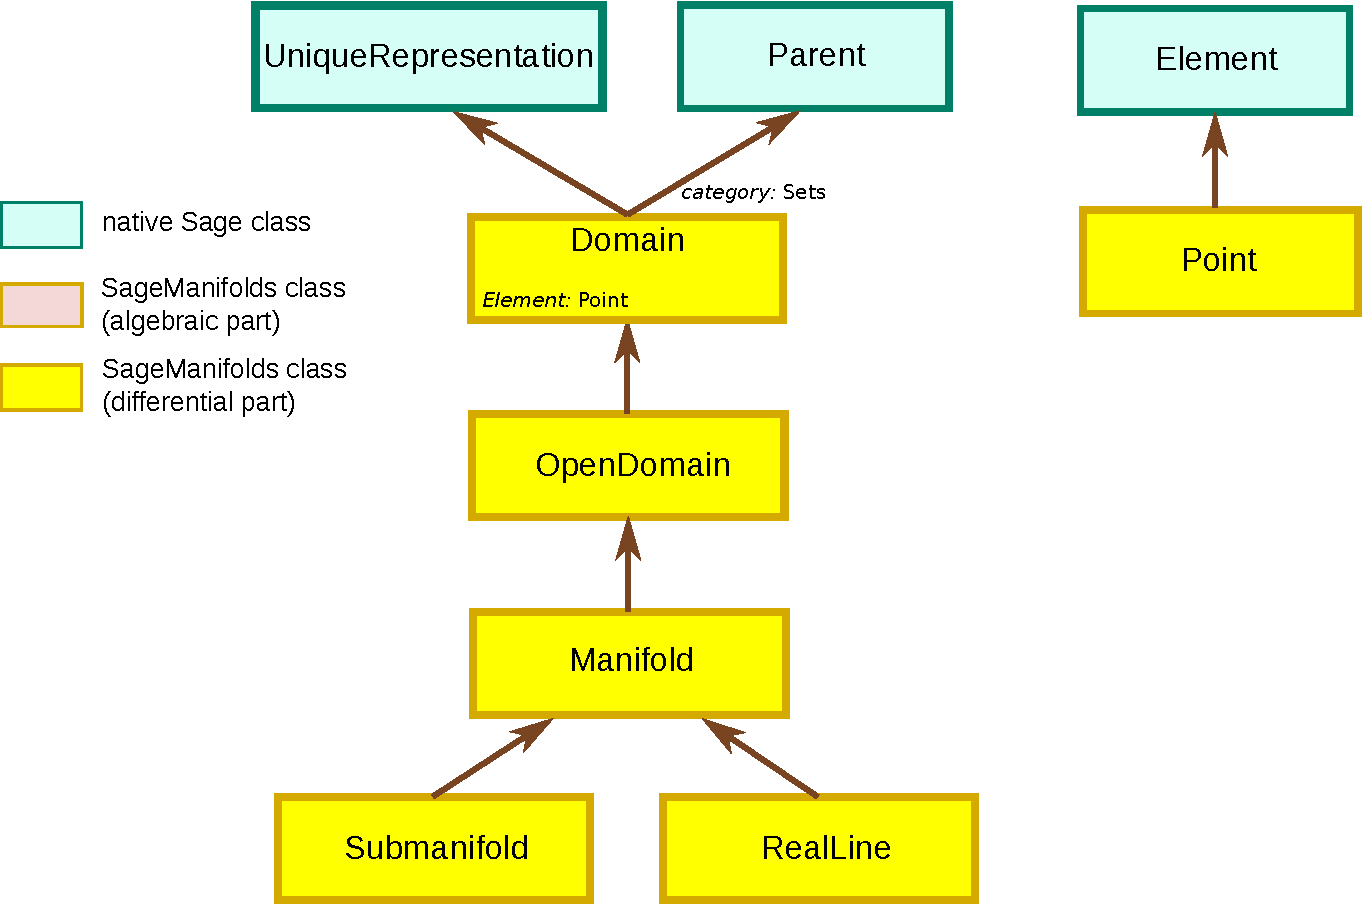
\includegraphics[width=0.7\textwidth]{domain_classes.pdf}
\end{center}
\caption{\label{f:domain_classes} Python classes for 
smooth manifolds (\code{Manifold}), generic subsets of them 
(\code{Domain}), open subsets of them (\code{OpenDomain})
and points on them (\code{Point}).}
\end{figure}

\subsection{Implementation of charts}

Given a manifold $\mathcal{M}$ of dimension $n$, a coordinate chart 
on an open subset $U\subset\mathcal{M}$ is implemented in \SM{} 
via the class \code{Chart}, whose main data is 
a $n$-tuple of \Sage{} symbolic variables $(x_1,\ldots,x_n)$, each of 
them representing a coordinate.
In general, more than one (regular) chart is required to cover the entire manifold.
For instance, at least 2 charts are necessary for the $n$-dimensional sphere 
$\mathbb{S}^n$ ($n\geq 1$), 3 charts for the real projective plane
$\mathbb{RP}^2$, and 4 charts for the torus $\mathbb{T}^2$. 
\SM{} allows for an arbitrary number of charts. 
To fully specify the manifold, one shall also provide the transition maps
(changes of coordinates) on
overlapping chart domains (\SM{} class \code{CoordChange}).


\subsection{Implementation of scalar fields}

A \emph{scalar field} on manifold $\mathcal{M}$ is a smooth mapping
\be
    \begin{array}{lcll}
    f: & U\subset \mathcal{M}&\longrightarrow &\mathbb{R} \\
       & p & \longmapsto  & f(p) ,
    \end{array}
\ee
where $U$ is an open subset of $\mathcal{M}$.
Note that a scalar field maps \emph{points}, not \emph{coordinates}, to real numbers. 
A scalar field $f$ has different coordinate representations $F$, $\hat F$, etc. 
in different charts $X$, $\hat X$, etc. defined on $U$:
\be
    f(p) = 
F(\underbrace{x^1,\ldots, x^n}_{\mbox{coord. of $p$}\atop\mbox{in chart $X$}}) 
= {\hat F}(\underbrace{{\hat x}^1,\ldots, {\hat x}^n}_{\mbox{coord. of $p$}\atop\mbox{in chart $\hat X$}})
= \ldots
\ee
These representations are 
stored in an attribute of the class \code{ScalarField}, a 
Python dictionary\footnote{A \emph{dictionary}, also known as \emph{associative array}, is a 
data structure that generalizes the concept of array in the sense that the
key to access to some element is not restricted to an integer or a tuple of integers.} 
whose keys are the charts:
\be \label{e:f_express}
 f.\mbox{\texttt{\_express}} = \left\{ X: F,\ \hat X: \hat F, \ldots \right\} .
\ee
Each representation $F$ is an instance of the class \code{FunctionChart}, 
which resembles \Sage{} native symbolic functions, but involves 
automatic simplifications in all arithmetic operations. 

\begin{figure}
\begin{center}
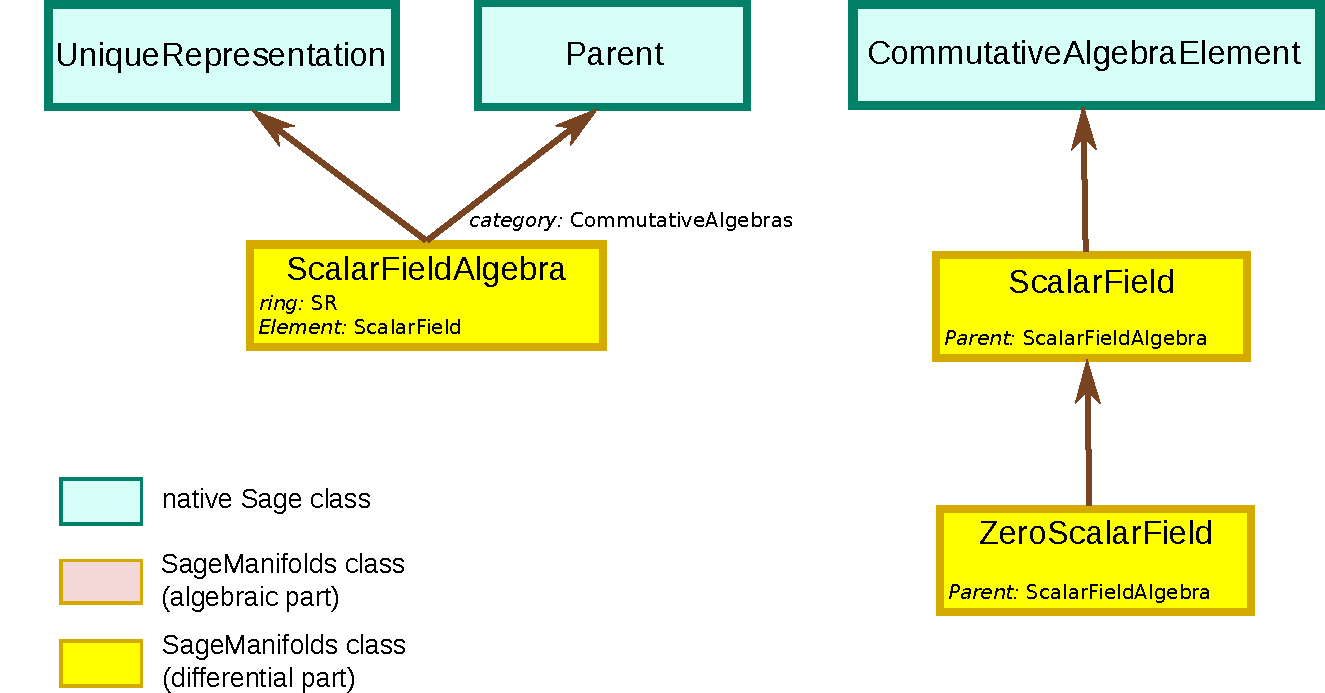
\includegraphics[width=0.7\textwidth]{scalar_classes.pdf}
\end{center}
\caption{\label{f:scalar_classes} Python classes for scalar fields
on a manifold.}
\end{figure}

Given an open subset $U\subset\mathcal{M}$, the set $C^\infty(U)$
of scalar fields defined on $U$ has naturally the structure of a 
commutative algebra over $\mathbb{R}$: it is clearly a vector
space over $\mathbb{R}$ and it is endowed with a commutative ring structure
by pointwise multiplication:
\be
\forall f, g \in C^\infty(U),\quad \forall p\in U,\quad
(f.g)(p) := f(p) g(p) .
\ee
The algebra $C^\infty(U)$ is implemented in \SM{} via the parent
class \code{ScalarFieldAlgebra}, in the category
\code{CommutativeAlgebras}. The corresponding element class 
is \code{ScalarField} (cf., Fig.~\ref{f:scalar_classes}). 

\subsection{Modules and free modules} \label{s:modules}

Given an open subset $U\subset\mathcal{M}$, the set $\mathcal{X}(U)$
of all smooth vector fields defined on $U$ has naturally the structure of a 
\emph{module over the algebra} $C^\infty(U)$.
Let us recall that a \emph{module} is similar to a \emph{vector space}, except that it is based
on a \emph{ring} (here $C^\infty(U)$)
instead of a \emph{field} (usually $\mathbb{R}$ or
$\mathbb{C}$ in physical applications). Of course, since every field is a ring, every vector space is a module.
There is an importance difference though: every vector space has a basis (as a 
consequence of the axiom of choice),
while a module does not necessarily have any. 
When it has one, it is called a \emph{free module}. 
Moreover, if the module's base ring is commutative, all bases have the same
cardinality, which is called the \emph{rank} of the module 
(for vector spaces, which are free modules, the word \emph{dimension}
is used instead of \emph{rank}). 

If $\mathcal{X}(U)$ is a free module, its basis is a \emph{vector frame}
$(\w{e}_a)_{1\leq a \leq n}$ on $U$:
\be \label{e:v_expand}
    \forall \w{v}\in\mathcal{X}(U),\quad \w{v} = v^a \w{e}_a,\quad\mbox{with\ } v^a \in C^\infty(U) .
\ee
The rank of $\mathcal{X}(U)$ is thus $n$, i.e., the manifold's 
dimension\footnote{Note that the dimensionality of $\mathcal{X}(U)$ depends
of the structure adopted for it: as a vector space over $\mathbb{R}$, the
dimension of $\mathcal{X}(U)$ is infinite, while as a free module over
$C^\infty(U)$, $\mathcal{X}(U)$ has a finite rank. Note also that if $\mathcal{X}(U)$
is not free (no global vector frame exists on $U$), the notion of rank 
is meaningless.}.

At any point $p\in U$, Eq.~(\ref{e:v_expand}) translates into an identity in 
the tangent vector space $T_p \mathcal{M}$:
\be 
    \w{v}(p) = v^a(p)  \; \w{e}_a(p),\quad\mbox{with\ } v^a(p) \in \mathbb{R} , 
\ee
which means that 
the set $(\w{e}_a(p))_{1\leq a \leq n}$ is a basis of the vector space $T_p \mathcal{M}$.
This is the very definition of a vector frame on $U$ (often called a \emph{tetrad} in
the context of 4-dimensional general relativity). Note that if $U$ is covered
by a chart $(x^a)_{1\leq a \leq n}$, then $(\partial/\partial x^a)_{1\leq a \leq n}$
is a vector frame on $U$, usually called \emph{coordinate frame}
or \emph{natural basis}. 


Another kind of free modules which occur naturally in the current context
is that of the tangent spaces to manifold $\mathcal{M}$: 
for each $p\in \mathcal{M}$, $T_p\mathcal{M}$ is a free module over 
$\mathbb{R}$, since it is a vector space over $\mathbb{R}$. 

It turns out that so far only \emph{free modules} with a distinguished basis were 
implemented in \Sage{}. This means that, given a free module $M$ of rank $n$, 
all calculations refer to a single basis of $M$. This amounts to identifying
$M$ with $R^n$, where $R$ is the ring over which $M$ is based. 
Current \Sage{} implementation is unfortunately 
not sufficient for dealing with generic manifolds in a coordinate-independent way. 
For instance, there is no canonical 
isomorphism between $T_p\mathcal{M}$ and $\mathbb{R}^n$ when no coordinate
system is privileged in the neighborhood of $p$.
Therefore we have started a pure algebraic branch of \SM{} to implement
generic free modules, with an arbitrary number of bases in them, 
none of them being distinguished. This resulted in the parent class 
\code{FiniteRankFreeModule}, in the category \code{Modules}, and in the element class 
\code{FiniteRankFreeModuleElement}. Then both the classes
\code{VectorFieldFreeModule} (for $\mathcal{X}(U)$, when it is 
a free module) and \code{TangentSpace} (for $T_p\mathcal{M}$)
inherit from \code{FiniteRankFreeModule} (see Fig.~\ref{f:module_classes}). 


\begin{figure}
\begin{center}
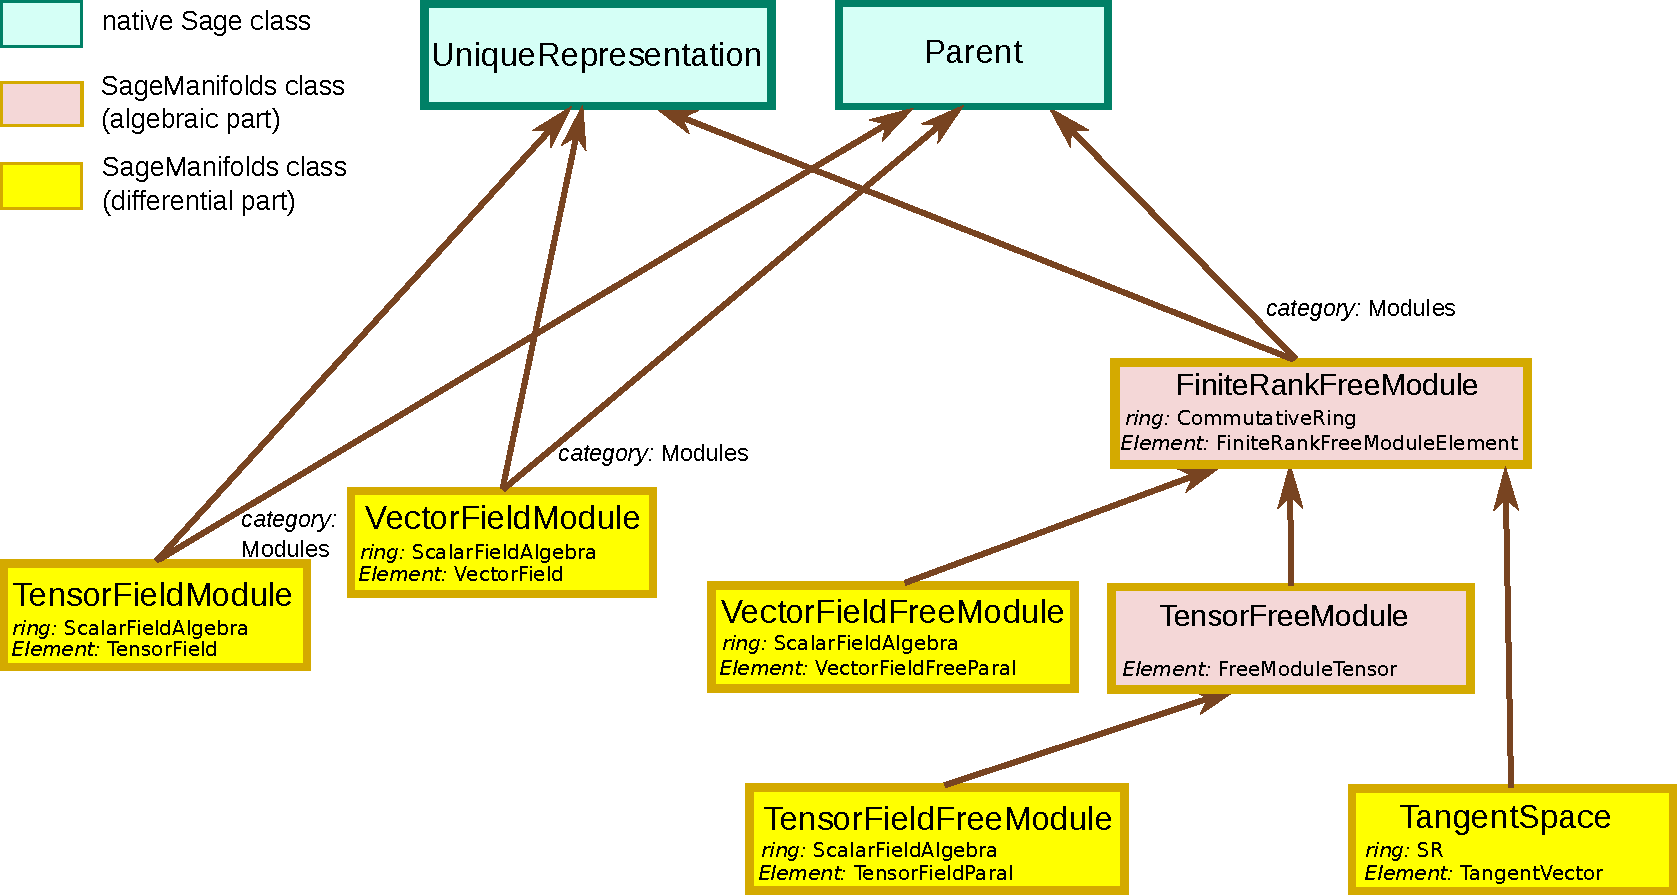
\includegraphics[width=0.8\textwidth]{module_classes.pdf}
\end{center}
\caption{\label{f:module_classes} Various module classes.}
\end{figure}



\subsection{Implementation of vector fields}

Ultimately, in \SM{}, vector fields are to be described by their 
components with respect to various vector frames, according to 
Eq.~(\ref{e:v_expand}), but without any vector frame being privileged, 
leaving the freedom to select them to the user, as well as to change 
coordinates. A key point is that 
not every manifold admits a global vector frame. 
A manifold $\mathcal{M}$, or more generally an open subset $U\subset\mathcal{M}$,
that admits a global vector frame is called 
\emph{parallelizable}. Equivalently,
$\mathcal{M}$ is parallelizable if, and only if, $\mathcal{X}(\mathcal{M})$
is a free module. In terms of the tangent bundle, 
parallelizable manifolds are those for which the tangent bundle is trivial:
$T\mathcal{M} \simeq \mathcal{M}\times \mathbb{R}^n$.
Examples of parallelizable manifolds are \cite{Lee13}
\begin{itemize}
\item the Cartesian space $\mathbb{R}^n$ for $n=1,2,\ldots$, 
\item the circle $\mathbb{S}^1$, 
\item the torus $\mathbb{T}^2 = \mathbb{S}^1\times \mathbb{S}^1$, 
\item the 3-sphere $\mathbb{S}^3 \simeq \mathrm{SU}(2)$, as any Lie group, 
\item the 7-sphere $\mathbb{S}^7$, 
\item any orientable 3-manifold (Steenrod theorem \cite{Steen51}).
\end{itemize}
On the other hand, examples of non-parallelizable manifolds are
\begin{itemize}
\item the sphere $\mathbb{S}^2$ (hairy ball theorem!) and any $n$-sphere $\mathbb{S}^n$ with $n\not\in\{1,3,7\}$, 
\item the real projective plane $\mathbb{RP}^2$.
\end{itemize}
Actually, ``most'' manifolds are non-parallelizable. 
As noticed above, if a manifold is covered by a single chart, it is 
parallelizable (the prototype being $\mathbb{R}^n$). But the reverse is not 
true: $\mathbb{S}^1$ and $\mathbb{T}^2$ are parallelizable and require 
at least two and four charts to cover them, respectively. 

\begin{figure}
\begin{center}
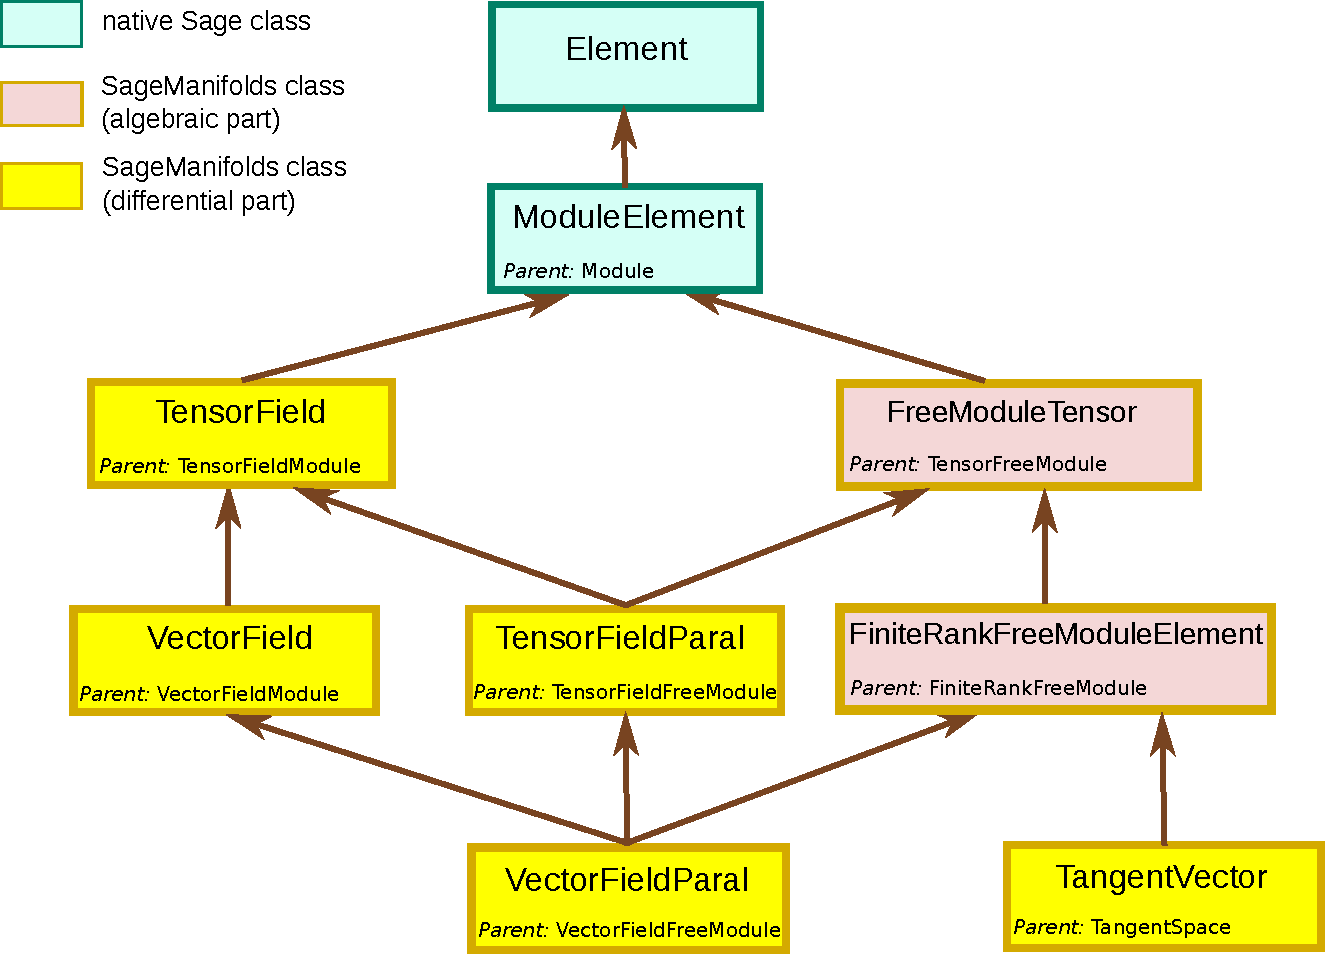
\includegraphics[width=0.7\textwidth]{tensorfield_classes.pdf}
\end{center}
\caption{\label{f:tensor_classes} Tensor and tensor field classes.}
\end{figure}

If the manifold $\mathcal{M}$ is not parallelizable, one has to decompose it 
into parallelizable
open subsets $U_i$ ($1\leq i \leq N$) 
and consider the restrictions of vector fields to these domains.
For each $i$, $\mathcal{X}(U_i)$ is a free module of rank $n=\mathrm{dim}\, \mathcal{M}$ and is implemented in \SM{} as an instance of 
\code{VectorFieldFreeModule} (cf., Sec.~\ref{s:modules} and Figs.~\ref{f:module_classes}
and \ref{f:tensor_classes}). 
Each vector field $\w{v}\in  \mathcal{X}(U_i)$ has different set
of components $(v^a)_{1\leq a\leq n}$ in different vector frames 
$(\w{e}_a)_{1\leq a \leq n}$ introduced on $U_i$ (cf., Eq.~\ref{e:v_expand}). They are stored
as a Python dictionary whose keys are the vector frames:
\be
\w{v}.\mbox{\texttt{\_components}} = \left\{ (\w{e}): (v^a),
\ (\w{\hat e}): ({\hat v}^a), \ldots \right\}. 
\ee


\subsection{Implementation of tensor fields}

The implementation of tensor fields in \SM{} follows the strategy 
adopted for vector fields. Consider for instance a tensor field $\w{T}$ 
of type-(1,1) on the manifold $\mathcal{M}$. 
It can be represented by 
components $T^a_{\ \, b}$ only on a parallelizable open subset $U\subset
\mathcal{M}$, since the decomposition 
\be \label{e:T_expand}
    \left. \w{T} \right| _{U} = T^a_{\ \, b} \, \w{e}_a \otimes \w{e}^b
\ee
that defines $T^a_{\ \, b}$ is meaningful only when a vector frame 
$(\w{e}_a)$ exist\footnote{Using standard notation, in Eq.~(\ref{e:T_expand})
$(\w{e}^b)$ stands for the coframe dual to $(\w{e}_a)$}.
Therefore, one first decomposes the tensor field $\w{T}$  into 
its restrictions $\left. \w{T} \right| _{U_i}$ on parallelizable open subsets
of $\mathcal{M}$, $U_i$ ($1\leq i\leq N$) and then considers 
the components on various vector frames on each subset $U_i$. 
This is illustrated in Fig.~\ref{f:tensorfield_structure}, which details the
internal storage of tensor fields in \SM{}. Note that each component
$T^a_{\ \, b}$ is a scalar field on $U_i$, according to the formula
\be
    T^a_{\ \, b} = \w{T}(\w{e}^a, \w{e}_b) . 
\ee
Accordingly, the penultimate level of Fig.~\ref{f:tensorfield_structure} 
corresponds to the scalar field storage, as described by (\ref{e:f_express}).
The last (bottom) level is constituted by \Sage{}'s symbolic expressions. 

\begin{figure}
\begin{center}
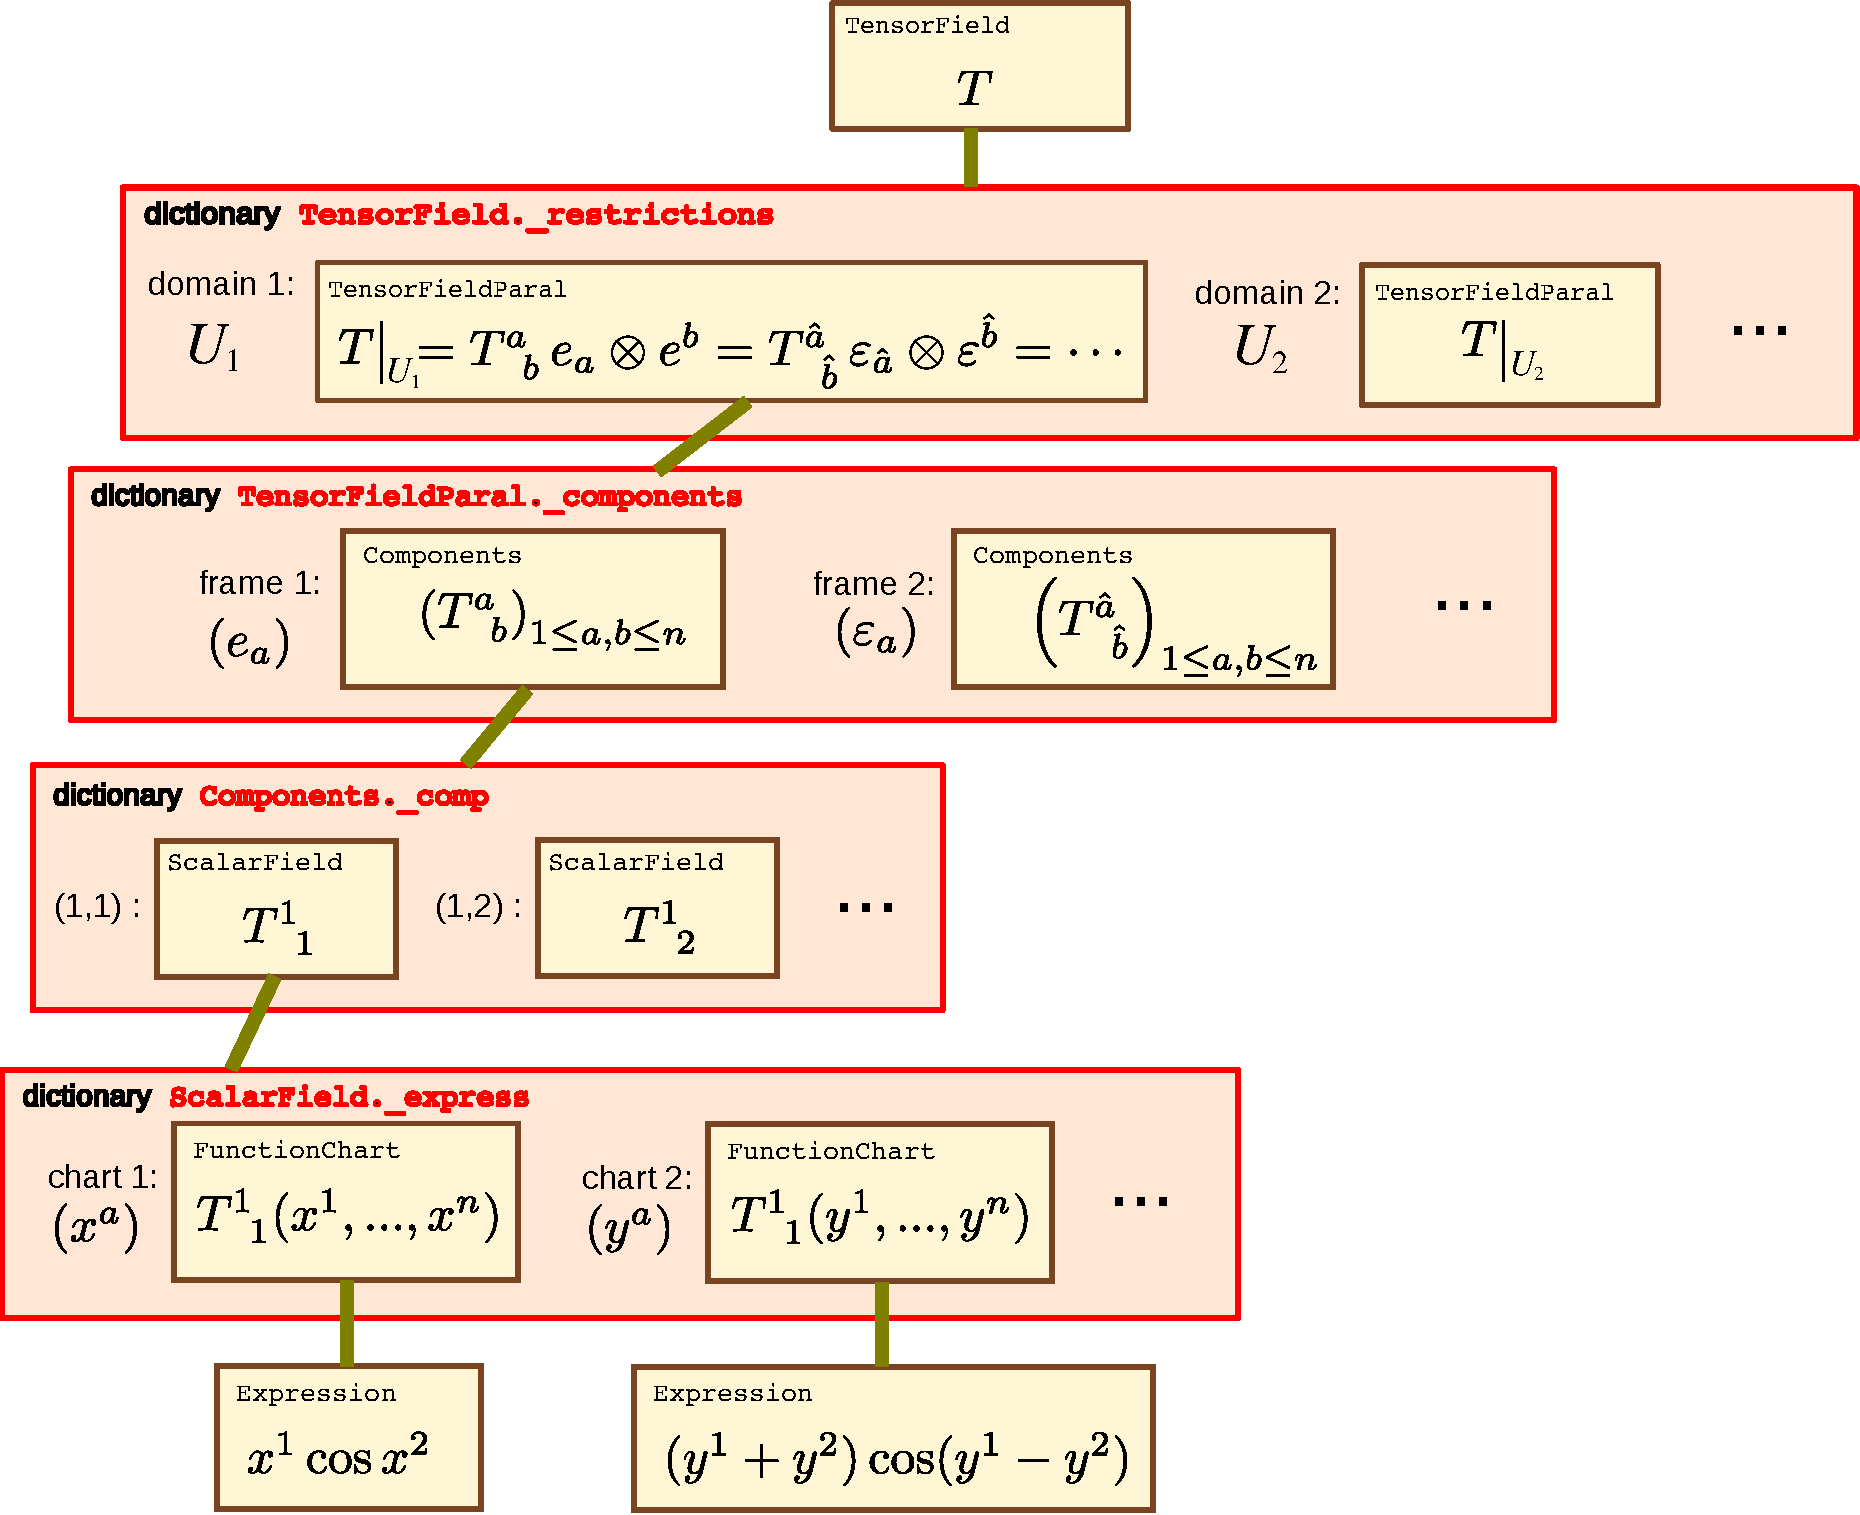
\includegraphics[width=0.8\textwidth]{tensorfield_structure.pdf}
\end{center}
\caption{\label{f:tensorfield_structure} Storage of tensor fields.}
\end{figure}



%%%%%%%%%%%%%%%%%%%%%%%%%%%%%%%%%%%%%%%%%%%%%%%%%%%%%%%%%

\section{Current status of SageManifolds}

\subsection{Functionalities} \label{s:functionalities}
At present (version 0.6), the functionalities included in \SM{} are as
follows:  
\begin{itemize}
\item maps between manifolds, pullback operator,
\item submanifolds, pushforward operator,
\item standard tensor calculus (tensor product, 
contraction, symmetrization, etc.), even on non-parallelizable manifolds,
\item taking in charge all monoterm tensor symmetries, 
\item exterior calculus (wedge product and exterior derivative of differential forms,
Hodge duality),
\item Lie derivatives,
\item affine connections (curvature, torsion),
\item pseudo-Riemannian metrics (Levi-Civita connection, Weyl tensor),
\item graphical display of charts.
\end{itemize}

\subsection{Parallelization}


%% Computationally demanding operations have been recently parallelized 
%% by means of the Python package \code{multiprocessing}, which is
%% implemented in \Sage{} via the decorator \code{@parallel}. 
%% The parallelization regards the arithmetic and contractions 
%% of tensors, the computation of connection coefficients and the computation
%% of the Riemann tensor. 

To improve the reactivity of \SM{} and take advantage of
the recent multicore processors, some tensorial operations are performed by
parallel processes. The parallelization is done using the built-in
\Sage{} decorator \code{Parallel}, which permits to define a function
that will be run on different sub-processes 
\footnote{The \code{Parallel} class is actually a wrap of the python library
\code{multiprocessing}.}. If $n$ processes are used, given a function
and a list of arguments for it, any process will call the function
with an element of the list, one at time, spanning all the list.

The parallelized tensorial operations are: tensorial algebra, tensor
contraction, affine connection and Riemann's tensor computation. 

The parallelization of an operation is done by first creating a
function which computes the required operation on a subset of the
components of a tensor; second, by creating a list of $2n$ (twice the
number of used processes) arguments for this function. Then applying this function
to the input list, the calculation will be done in parallel. 
At the end of the computation a fourth phase is needed to retrieve the
results.
The choice to divide the work in $2n$ is a compromise between a better
load balancing and cost of create multiple processes.

The number of processors used in the parallelization is controlled by
the global variable \code{manifoldPara} which member fuction \code{set}
permits to fix the number of processes to use.

This feature shall be available in version 0.7. 


%%%%%%%%%%%%%%%%%%%%%%%%%%%%%%%%%%%%%%%%%%%%%%%%%%%%%%%%%

\section{SageManifolds at work: Kerr spacetime and Simon-Mars tensor}

We give hereafter a short illustration of \SM{} focused on tensor 
calculus. Another example, based on the sphere $\mathbb{S}^2$, 
focusses more on the use of multiple charts and the treatment of non-parallelizable 
manifolds. This example and many others are available at
\cite{SM_examples}.

Let us consider a 4-dimensional spacetime, i.e., a 4-dimensional smooth 
manifold $\mathcal{M}$ endowed with a Lorentzian metric $\w{g}$. 
We assume that the spacetime is stationary and denote by $\w{\xi}$ 
the corresponding Killing vector field. 
The \emph{Simon-Mars tensor w.r.t. $\w{\xi}$} is then
the type-(0,3) tensor field $\w{S}$ defined by 
\be \label{e:def_Simon-Mars}
S_{\alpha\beta\gamma} := 4 \mathcal{C}_{\mu\alpha\nu[\beta} \, \xi^\mu \xi^\nu \, \sigma_{\gamma]}
 + \gamma_{\alpha[\beta} \, \mathcal{C}_{\gamma]\rho\mu\nu} \, \xi^\rho \, \mathcal{F}^{\mu\nu} ,
\ee
where
\begin{itemize}
\item $\gamma_{\alpha\beta} := \lambda \, g_{\alpha\beta} + \xi_\alpha \xi_\beta$, 
with $\lambda := - \xi_\mu \xi^\mu$
\item $\mathcal{C}_{\alpha\beta\mu\nu} := C_{\alpha\beta\mu\nu}
    + \frac{i}{2} \epsilon^{\rho\sigma}_{\ \ \, \mu\nu}\,  C_{\alpha\beta\rho\sigma} $,
with $C^\alpha_{\ \, \beta\mu\nu}$ being the Weyl tensor and 
$\epsilon_{\alpha\beta\mu\nu}$ the Levi-Civita volume form
\item $\mathcal{F}_{\alpha\beta} := F_{\alpha\beta} + i\,  {}^*\!F_{\alpha\beta}$, 
with $F_{\alpha\beta} := \nabla_\alpha\xi_\beta$ (Killing 2-form) and 
${}^*\!F_{\alpha\beta} := \frac{1}{2} \epsilon^{\mu\nu}_{\ \ \, \alpha\beta} F_{\mu\nu}$
(Hodge dual of $F_{\alpha\beta}$)
\item $\sigma_\alpha := 2 \mathcal{F}_{\mu\alpha} \xi^\mu$ (Ernst 1-form)
\end{itemize}
As shown by Mars \cite{Mars99}, the 
Simon-Mars tensor provides a nice characterization of Kerr spacetime:
if $\w{g}$ satisfies the vacuum Einstein equation and $(\mathcal{M},\w{g})$
contains a stationary asymptotically flat end $\mathcal{M}^\infty$ such
that $\w{\xi}$ tends to a time translation at infinity in $\mathcal{M}^\infty$
and the Komar mass of $\w{\xi}$ in $\mathcal{M}^\infty$ is non-zero, then 
$\w{S} = 0$ if, and only if, $(\mathcal{M},\w{g})$ is locally isometric 
to a Kerr spacetime.

In what follows, we use \SM{} to compute the Simon-Mars tensor 
according to formula (\ref{e:def_Simon-Mars}) for the Kerr metric and check 
that we get zero, which is not trivial. 
The corresponding worksheet can be downloaded from \\
\url{http://sagemanifolds.obspm.fr/examples/html/SM_Mars-Simon.html}.\\
To fully understand what follows, the reader must be aware that, 
as an object-oriented language, Python (and hence \Sage{}) makes use of 
the following postfix notation:
\begin{center}
\textcolor{blue}{\texttt{result}} = \textcolor{red}{\texttt{object}}\texttt{.}\texttt{function(}\textcolor{green}{\texttt{arguments}}\texttt{)}
\end{center}
In a functional language, this would be written instead as
 \begin{center}
\textcolor{blue}{\texttt{result}} = \texttt{function(}\textcolor{red}{\texttt{object}}\texttt{,}\textcolor{green}{\texttt{arguments}}\texttt{)}
\end{center}
For instance, the Riemann tensor of a metric $g$ is obtained as 
\begin{verbatim}
riem = g.riemann()
\end{verbatim}
In this case, there is no extra argument, hence the empty parentheses. 
With this is mind, let us proceed with the computation by means of 
\SM{}. 

The first step is to declare the Kerr spacetime (or more precisely the part of the Kerr spacetime covered by Boyer-Lindquist coordinates) as a 4-dimensional manifold:
\begin{verbatim}
M = Manifold(4, 'M', latex_name=r'\mathcal{M}')
print M
\end{verbatim}
\soutput{4-dimensional manifold 'M'}
We introduce the standard Boyer-Lindquist coordinates $(t,r,\theta,\phi)$
by declaring a chart $X$ on $\mathcal{M}$:
\begin{verbatim}
X.<t,r,th,ph> = M.chart(r't r:(0,+oo) th:(0,pi):\theta ph:(0,2*pi):\phi') 
print X ; X
\end{verbatim}
\soutput{chart (M, (t, r, th, ph))\\
$(\mathcal{M},(t, r, \theta, \phi))$}
We define next the Kerr metric $g$ by setting its components in the 
coordinate frame associated with Boyer-Lindquist coordinates, 
which is the current manifold's default frame:
\begin{verbatim}
g = M.lorentz_metric('g')
m = var('m') ; a = var('a')
rho2 = r^2 + (a*cos(th))^2
Delta = r^2 -2*m*r + a^2
g[0,0] = -(1-2*m*r/rho2)
g[0,3] = -2*a*m*r*sin(th)^2/rho2
g[1,1], g[2,2] = rho2/Delta, rho2
g[3,3] = (r^2+a^2+2*m*r*(a*sin(th))^2/rho2)*sin(th)^2
g.view()
\end{verbatim}
\soutput{$\displaystyle g = \left( -\frac{a^{2} \cos\left(\theta\right)^{2} - 2 \, m r +
r^{2}}{a^{2} \cos\left(\theta\right)^{2} + r^{2}} \right) \mathrm{d}
t\otimes \mathrm{d} t + \left( -\frac{2 \, a m r
\sin\left(\theta\right)^{2}}{a^{2} \cos\left(\theta\right)^{2} + r^{2}}
\right) \mathrm{d} t\otimes \mathrm{d} \phi \ + $\\
$\displaystyle \left( \frac{a^{2}
\cos\left(\theta\right)^{2} + r^{2}}{a^{2} - 2 \, m r + r^{2}} \right)
\mathrm{d} r\otimes \mathrm{d} r + \left( a^{2}
\cos\left(\theta\right)^{2} + r^{2} \right) \mathrm{d} \theta\otimes
\mathrm{d} \theta + \left( -\frac{2 \, a m r
\sin\left(\theta\right)^{2}}{a^{2} \cos\left(\theta\right)^{2} + r^{2}}
\right) \mathrm{d} \phi\otimes \mathrm{d} t + \left( \frac{2 \, a^{2} m
r \sin\left(\theta\right)^{4} + {\left(a^{2} r^{2} + r^{4} +
{\left(a^{4} + a^{2} r^{2}\right)} \cos\left(\theta\right)^{2}\right)}
\sin\left(\theta\right)^{2}}{a^{2} \cos\left(\theta\right)^{2} + r^{2}}
\right) \mathrm{d} \phi\otimes \mathrm{d} \phi $}
The Levi-Civita connection $\nabla$ associated with g is obtained
by the method \code{connection()}:
\begin{verbatim}
nab = g.connection() ; print nab
\end{verbatim}
\soutput{Levi-Civita connection 'nabla\_g' associated with the Lorentzian metric
'g' on the 4-dimensional manifold 'M'}
As a check, we verify that the covariant derivative of $g$ with respect to
$\nabla$ vanishes identically:
\begin{verbatim}
nab(g).view()
\end{verbatim}
\soutput{$ \nabla_{g} g = 0$}
The default vector frame on the spacetime manifold is the coordinate basis associated with Boyer-Lindquist coordinates:
\begin{verbatim}
M.default_frame() is X.frame()
\end{verbatim}
\soutput{True}
\begin{verbatim}
X.frame()
\end{verbatim}
\soutput{$\left(\mathcal{M} ,\left(\frac{\partial}{\partial t
},\frac{\partial}{\partial r },\frac{\partial}{\partial \theta
},\frac{\partial}{\partial \phi }\right)\right)$}
Let us consider the first vector field of this frame:
\begin{verbatim}
xi = X.frame()[0] ; xi
\end{verbatim}
\soutput{$\frac{\partial}{\partial t}$}
\begin{verbatim}
print xi 
\end{verbatim}
\soutput{vector field 'd/dt' on the 4-dimensional manifold 'M'}
The 1-form associated to it by metric duality is
\begin{verbatim}
xi_form = xi.down(g)
xi_form.set_name('xi_form', r'\underline{\xi}')
print xi_form ; xi_form.view()
\end{verbatim}
\soutput{1-form 'xi\_form' on the 4-dimensional manifold 'M'\\[1ex]
$\underline{\xi} = \left( -\frac{a^{2} \cos\left(\theta\right)^{2} - 2 \,
m r + r^{2}}{a^{2} \cos\left(\theta\right)^{2} + r^{2}} \right)
\mathrm{d} t + \left( -\frac{2 \, a m r
\sin\left(\theta\right)^{2}}{a^{2} \cos\left(\theta\right)^{2} + r^{2}}
\right) \mathrm{d} \phi$}
Its covariant derivative is
\begin{verbatim}
nab_xi = nab(xi_form)
print nab_xi ; nab_xi.view()
\end{verbatim}
\soutput{tensor field 'nabla\_g xi\_form' of type (0,2) on the 4-dimensional
manifold 'M'\\[1ex]
$\nabla_{g} \underline{\xi} = \left( \frac{a^{2} m
\cos\left(\theta\right)^{2} - m r^{2}}{a^{4} \cos\left(\theta\right)^{4}
+ 2 \, a^{2} r^{2} \cos\left(\theta\right)^{2} + r^{4}} \right)
\mathrm{d} t\otimes \mathrm{d} r + \left( \frac{2 \, a^{2} m r
\cos\left(\theta\right) \sin\left(\theta\right)}{a^{4}
\cos\left(\theta\right)^{4} + 2 \, a^{2} r^{2}
\cos\left(\theta\right)^{2} + r^{4}} \right) \mathrm{d} t\otimes
\mathrm{d} \theta + $\\
$\left( -\frac{a^{2} m \cos\left(\theta\right)^{2} -
m r^{2}}{a^{4} \cos\left(\theta\right)^{4} + 2 \, a^{2} r^{2}
\cos\left(\theta\right)^{2} + r^{4}} \right) \mathrm{d} r\otimes
\mathrm{d} t + \left( \frac{{\left(a^{3} m \cos\left(\theta\right)^{2} -
a m r^{2}\right)} \sin\left(\theta\right)^{2}}{a^{4}
\cos\left(\theta\right)^{4} + 2 \, a^{2} r^{2}
\cos\left(\theta\right)^{2} + r^{4}} \right) \mathrm{d} r\otimes
\mathrm{d} \phi + $\\
$\left( -\frac{2 \, a^{2} m r \cos\left(\theta\right)
\sin\left(\theta\right)}{a^{4} \cos\left(\theta\right)^{4} + 2 \, a^{2}
r^{2} \cos\left(\theta\right)^{2} + r^{4}} \right) \mathrm{d}
\theta\otimes \mathrm{d} t + \left( \frac{2 \, {\left(a^{3} m r + a m
r^{3}\right)} \cos\left(\theta\right) \sin\left(\theta\right)}{a^{4}
\cos\left(\theta\right)^{4} + 2 \, a^{2} r^{2}
\cos\left(\theta\right)^{2} + r^{4}} \right) \mathrm{d} \theta\otimes
\mathrm{d} \phi + $ \\
$\left( -\frac{{\left(a^{3} m
\cos\left(\theta\right)^{2} - a m r^{2}\right)}
\sin\left(\theta\right)^{2}}{a^{4} \cos\left(\theta\right)^{4} + 2 \,
a^{2} r^{2} \cos\left(\theta\right)^{2} + r^{4}} \right) \mathrm{d}
\phi\otimes \mathrm{d} r + \left( -\frac{2 \, {\left(a^{3} m r + a m
r^{3}\right)} \cos\left(\theta\right) \sin\left(\theta\right)}{a^{4}
\cos\left(\theta\right)^{4} + 2 \, a^{2} r^{2}
\cos\left(\theta\right)^{2} + r^{4}} \right) \mathrm{d} \phi\otimes
\mathrm{d} \theta$}
Let us check that the Killing equation is satisfied:
\begin{verbatim}
nab_xi.symmetrize().view()
\end{verbatim}
\soutput{$0$}
Equivalently, we check that the Lie derivative of the metric along $\xi$
vanishes:
\begin{verbatim}
g.lie_der(xi).view()
\end{verbatim}
\soutput{$0$}
Thanks to Killing equation, $\nabla_g \underline{\xi}$ is antisymmetric. We may therefore define a 2-form by $F:= - \nabla_g \underline{\xi}$. Here we enforce the antisymmetry by calling the method \code{antisymmetrize()} on \code{nab\_xi}:
\begin{verbatim}
F = - nab_xi.antisymmetrize()
F.set_name('F')
print F ; F.view()
\end{verbatim}
\soutput{2-form 'F' on the 4-dimensional manifold 'M'\\[1ex]
$F = \left( -\frac{a^{2} m \cos\left(\theta\right)^{2} - m r^{2}}{a^{4}
\cos\left(\theta\right)^{4} + 2 \, a^{2} r^{2}
\cos\left(\theta\right)^{2} + r^{4}} \right) \mathrm{d} t\wedge
\mathrm{d} r + \left( -\frac{2 \, a^{2} m r \cos\left(\theta\right)
\sin\left(\theta\right)}{a^{4} \cos\left(\theta\right)^{4} + 2 \, a^{2}
r^{2} \cos\left(\theta\right)^{2} + r^{4}} \right) \mathrm{d} t\wedge
\mathrm{d} \theta + $\\
$\left( -\frac{{\left(a^{3} m
\cos\left(\theta\right)^{2} - a m r^{2}\right)}
\sin\left(\theta\right)^{2}}{a^{4} \cos\left(\theta\right)^{4} + 2 \,
a^{2} r^{2} \cos\left(\theta\right)^{2} + r^{4}} \right) \mathrm{d}
r\wedge \mathrm{d} \phi + \left( -\frac{2 \, {\left(a^{3} m r + a m
r^{3}\right)} \cos\left(\theta\right) \sin\left(\theta\right)}{a^{4}
\cos\left(\theta\right)^{4} + 2 \, a^{2} r^{2}
\cos\left(\theta\right)^{2} + r^{4}} \right) \mathrm{d} \theta\wedge
\mathrm{d} \phi$}
The squared norm of the Killing vector is:
\begin{verbatim}
lamb = - g(xi,xi)
lamb.set_name('lambda', r'\lambda')
print lamb ; lamb.view()
\end{verbatim}
\soutput{scalar field 'lambda' on the 4-dimensional manifold 'M'\\[1ex]
$\begin{array}{llcl} \lambda:& \mathcal{M} & \longrightarrow
& \mathbb{R} \\ & \left(t, r, \theta, \phi\right) & \longmapsto
& \frac{a^{2} \cos\left(\theta\right)^{2} - 2 \, m r + r^{2}}{a^{2}
\cos\left(\theta\right)^{2} + r^{2}} \end{array}$\\[-1ex]}
Instead of invoking $g(\xi,\xi)$, we could have evaluated $\lambda$ 
by means of the 1-form $\underline{\xi}$ acting on the vector field $\xi$:
\begin{verbatim}
lamb == - xi_form(xi)
\end{verbatim}
\soutput{True}
or, using index notation,
\begin{verbatim}
lamb == - ( xi_form['_a']*xi['^a'] )
\end{verbatim}
\soutput{True}
The Riemann curvature tensor associated with $g$ is:
\begin{verbatim}
Riem = g.riemann()
print Riem
\end{verbatim}
\soutput{tensor field 'Riem(g)' of type (1,3) on the 4-dimensional manifold 'M'}
The component $R^0_{\ \, 123} = R^t_{\ \, r\theta\phi}$ is 
\begin{verbatim}
Riem[0,1,2,3]
\end{verbatim}
\soutput{\tiny $-\frac{{\left(a^{7} m - 2 \, a^{5} m^{2} r + a^{5} m r^{2}\right)}
\cos\left(\theta\right) \sin\left(\theta\right)^{5} + {\left(a^{7} m + 2
\, a^{5} m^{2} r + 6 \, a^{5} m r^{2} - 6 \, a^{3} m^{2} r^{3} + 5 \,
a^{3} m r^{4}\right)} \cos\left(\theta\right)
\sin\left(\theta\right)^{3} - 2 \, {\left(a^{7} m - a^{5} m r^{2} - 5 \,
a^{3} m r^{4} - 3 \, a m r^{6}\right)} \cos\left(\theta\right)
\sin\left(\theta\right)}{a^{2} r^{6} - 2 \, m r^{7} + r^{8} +
{\left(a^{8} - 2 \, a^{6} m r + a^{6} r^{2}\right)}
\cos\left(\theta\right)^{6} + 3 \, {\left(a^{6} r^{2} - 2 \, a^{4} m
r^{3} + a^{4} r^{4}\right)} \cos\left(\theta\right)^{4} + 3 \,
{\left(a^{4} r^{4} - 2 \, a^{2} m r^{5} + a^{2} r^{6}\right)}
\cos\left(\theta\right)^{2}}$}
The Ricci tensor vanishes identically, i.e., we check that the Kerr metric is 
a vacuum solution of Einstein equation:
\begin{verbatim}
g.ricci().view()
\end{verbatim}
\soutput{$\mathrm{Ric}(g) = 0$}
The Weyl conformal curvature tensor is
\begin{verbatim}
C = g.weyl() ; print C
\end{verbatim}
\soutput{tensor field 'C(g)' of type (1,3) on the 4-dimensional manifold 'M'}
Let us exhibit the component $C^0_{\ \, 101}=C^t_{\ \, rtr}$:
\begin{verbatim}
C[0,1,0,1]
\end{verbatim}
\soutput{$\frac{3 \, a^{4} m r \cos\left(\theta\right)^{4} + 3 \, a^{2} m r^{3} +
2 \, m r^{5} - {\left(9 \, a^{4} m r + 7 \, a^{2} m r^{3}\right)}
\cos\left(\theta\right)^{2}}{a^{2} r^{6} - 2 \, m r^{7} + r^{8} +
{\left(a^{8} - 2 \, a^{6} m r + a^{6} r^{2}\right)}
\cos\left(\theta\right)^{6} + 3 \, {\left(a^{6} r^{2} - 2 \, a^{4} m
r^{3} + a^{4} r^{4}\right)} \cos\left(\theta\right)^{4} + 3 \,
{\left(a^{4} r^{4} - 2 \, a^{2} m r^{5} + a^{2} r^{6}\right)}
\cos\left(\theta\right)^{2}}$}
To form the Simon-Mars tensor, we need the fully covariant (type-(0,4)
tensor) form of the Weyl tensor (i.e., $C_{\alpha\beta\mu\nu} = g_{\alpha\sigma} C^\sigma_{\ \, \beta\mu\nu}$); we get it by lowering the first index with the metric:
\begin{verbatim}
Cd = C.down(g) ; print Cd
\end{verbatim}
\soutput{tensor field of type (0,4) on the 4-dimensional manifold 'M'}
The (monoterm) symmetries of this tensor are those inherited from the
Weyl tensor, i.e., the antisymmetry on the last two indices (position 2 and 3, the first index being at position 0):
\begin{verbatim}
Cd.symmetries()
\end{verbatim}
\soutput{no symmetry;  antisymmetry: (2, 3)}
Actually, Cd is also antisymmetric with respect to the first two indices (positions 0 and 1), as we can check:
\begin{verbatim}
Cd == Cd.antisymmetrize(0,1)
\end{verbatim}
\soutput{True}
To take this symmetry into account explicitly, we set
\begin{verbatim}
Cd = Cd.antisymmetrize(0,1)
Cd.symmetries()
\end{verbatim}
\soutput{no symmetry;  antisymmetries: [(0, 1), (2, 3)]}
The starting point in the evaluation of Simon-Mars tensor is the
self-dual complex 2-form associated with the Killing 2-form $F$, i.e., the object $\mathcal{F} := F + i \, {}^* F$, where ${}^*F$ is the Hodge dual of $F$:
\begin{verbatim}
FF = F + I * F.hodge_star(g)
FF.set_name('FF', r'\mathcal{F}')
print FF ; FF.view()
\end{verbatim}
\soutput{2-form 'FF' on the 4-dimensional manifold 'M'\\
$\mathcal{F} = \left( -\frac{a^{2} m \cos\left(\theta\right)^{2} + 2 i \,
a m r \cos\left(\theta\right) - m r^{2}}{a^{4}
\cos\left(\theta\right)^{4} + 2 \, a^{2} r^{2}
\cos\left(\theta\right)^{2} + r^{4}} \right) \mathrm{d} t\wedge
\mathrm{d} r + \left( \frac{{\left(i \, a^{3} m
\cos\left(\theta\right)^{2} - 2 \, a^{2} m r \cos\left(\theta\right) - i
\, a m r^{2}\right)} \sin\left(\theta\right)}{a^{4}
\cos\left(\theta\right)^{4} + 2 \, a^{2} r^{2}
\cos\left(\theta\right)^{2} + r^{4}} \right) \mathrm{d} t\wedge
\mathrm{d} \theta + \left( \frac{-4 i \, a^{4} m^{2} r^{2}
\cos\left(\theta\right) \sin\left(\theta\right)^{4} + {\left(a^{3} m
r^{4} - 2 \, a m^{2} r^{5} + a m r^{6} - {\left(a^{7} m - 2 \, a^{5}
m^{2} r + a^{5} m r^{2}\right)} \cos\left(\theta\right)^{4} - {\left(2 i
\, a^{6} m r + 2 i \, a^{4} m r^{3}\right)} \cos\left(\theta\right)^{3}
- {\left(-4 i \, a^{4} m^{2} r^{2} + 2 i \, a^{4} m r^{3} - 4 i \, a^{2}
m^{2} r^{4} + 2 i \, a^{2} m r^{5}\right)}
\cos\left(\theta\right)\right)} \sin\left(\theta\right)^{2}}{a^{2} r^{6}
- 2 \, m r^{7} + r^{8} + {\left(a^{8} - 2 \, a^{6} m r + a^{6}
r^{2}\right)} \cos\left(\theta\right)^{6} + 3 \, {\left(a^{6} r^{2} - 2
\, a^{4} m r^{3} + a^{4} r^{4}\right)} \cos\left(\theta\right)^{4} + 3
\, {\left(a^{4} r^{4} - 2 \, a^{2} m r^{5} + a^{2} r^{6}\right)}
\cos\left(\theta\right)^{2}} \right) \mathrm{d} r\wedge \mathrm{d} \phi
+ \left( -\frac{{\left(i \, a^{4} m + i \, a^{2} m r^{2}\right)}
\sin\left(\theta\right)^{3} + {\left(-i \, a^{4} m + i \, m r^{4} + 2 \,
{\left(a^{3} m r + a m r^{3}\right)} \cos\left(\theta\right)\right)}
\sin\left(\theta\right)}{a^{4} \cos\left(\theta\right)^{4} + 2 \, a^{2}
r^{2} \cos\left(\theta\right)^{2} + r^{4}} \right) \mathrm{d}
\theta\wedge \mathrm{d} \phi$}
Let us check that $\mathcal{F}$ is self-dual, i.e., that it obeys ${}^* \mathcal{F} = -i \mathcal{F}$:
\begin{verbatim}
FF.hodge_star(g) == - I * FF
\end{verbatim}
\soutput{True}
To evaluate the right self-dual of the Weyl tensor, we need the 
tensor $\epsilon^{\alpha\beta}_{\ \ \ \gamma\delta}$:
\begin{verbatim}
eps = g.volume_form(2)  # 2 = the first 2 indices are contravariant
print eps ; eps.symmetries()
\end{verbatim}
\soutput{tensor field of type (2,2) on the 4-dimensional manifold 'M'\\
no symmetry;  antisymmetries: [(0, 1), (2, 3)]}
The right self-dual Weyl tensor is then:
\begin{verbatim}
CC = Cd + I/2*( eps['^rs_..']*Cd['_..rs'] )
CC.set_name('CC', r'\mathcal{C}') ; 
print CC ; CC.symmetries()
\end{verbatim}
\soutput{tensor field 'CC' of type (0,4) on the 4-dimensional manifold 'M'\\
no symmetry;  antisymmetries: [(0, 1), (2, 3)]}
\begin{verbatim}
CC[0,1,2,3]
\end{verbatim}
\soutput{$\frac{{\left(a^{5} m \cos\left(\theta\right)^{5} + 3 i \, a^{4} m r
\cos\left(\theta\right)^{4} + 3 i \, a^{2} m r^{3} + 2 i \, m r^{5} -
{\left(3 \, a^{5} m + 5 \, a^{3} m r^{2}\right)}
\cos\left(\theta\right)^{3} + {\left(-9 i \, a^{4} m r - 7 i \, a^{2} m
r^{3}\right)} \cos\left(\theta\right)^{2} + 3 \, {\left(3 \, a^{3} m
r^{2} + 2 \, a m r^{4}\right)} \cos\left(\theta\right)\right)}
\sin\left(\theta\right)}{a^{6} \cos\left(\theta\right)^{6} + 3 \, a^{4}
r^{2} \cos\left(\theta\right)^{4} + 3 \, a^{2} r^{4}
\cos\left(\theta\right)^{2} + r^{6}}$}
The Ernst 1-form $\sigma_\alpha = 2 \mathcal{F}_{\mu\alpha} \, \xi^\mu$ (0 = contraction on the first index of $\mathcal{F}$):
\begin{verbatim}
sigma = 2*FF.contract(0, xi)
\end{verbatim}
Instead of invoking the method \code{contract()}, 
we could have used the index notation to denote the contraction:
\begin{verbatim}
sigma == 2*( FF['_ma']*xi['^m'] )
\end{verbatim}
\soutput{True}
\begin{verbatim}
sigma.set_name('sigma', r'\sigma')
print sigma ; sigma.view()
\end{verbatim}
\soutput{1-form 'sigma' on the 4-dimensional manifold 'M'\\
$\sigma = \left( -\frac{2 \, a^{2} m \cos\left(\theta\right)^{2} + 4 i \,
a m r \cos\left(\theta\right) - 2 \, m r^{2}}{a^{4}
\cos\left(\theta\right)^{4} + 2 \, a^{2} r^{2}
\cos\left(\theta\right)^{2} + r^{4}} \right) \mathrm{d} r + \left(
\frac{{\left(2 i \, a^{3} m \cos\left(\theta\right)^{2} - 4 \, a^{2} m r
\cos\left(\theta\right) - 2 i \, a m r^{2}\right)}
\sin\left(\theta\right)}{a^{4} \cos\left(\theta\right)^{4} + 2 \, a^{2}
r^{2} \cos\left(\theta\right)^{2} + r^{4}} \right) \mathrm{d} \theta$}
The symmetric bilinear form $\gamma = \lambda \, g + \underline{\xi}\otimes\underline{\xi}$:
\begin{verbatim}
gamma = lamb*g + xi_form * xi_form
gamma.set_name('gamma', r'\gamma')
print gamma ; gamma.view()
\end{verbatim}
\soutput{field of symmetric bilinear forms 'gamma' on the 4-dimensional manifold
'M'\\
$\gamma = \left( \frac{a^{2} \cos\left(\theta\right)^{2} - 2 \, m r +
r^{2}}{a^{2} - 2 \, m r + r^{2}} \right) \mathrm{d} r\otimes \mathrm{d}
r + \left( a^{2} \cos\left(\theta\right)^{2} - 2 \, m r + r^{2} \right)
\mathrm{d} \theta\otimes \mathrm{d} \theta +$\\
$\left( \frac{2 \, a^{2} m r
\sin\left(\theta\right)^{4} - {\left(2 \, a^{2} m r - a^{2} r^{2} + 2 \,
m r^{3} - r^{4} - {\left(a^{4} + a^{2} r^{2}\right)}
\cos\left(\theta\right)^{2}\right)} \sin\left(\theta\right)^{2}}{a^{2}
\cos\left(\theta\right)^{2} + r^{2}} \right) \mathrm{d} \phi\otimes
\mathrm{d} \phi$}
The first part of the Simon-Mars tensor is 
$S^{(1)}_{\alpha\beta\gamma} = 4 \mathcal{C}_{\mu\alpha\nu\beta} \, \xi^\mu \, \xi^\nu \, \sigma_\gamma$:
\begin{verbatim}
S1 = 4*( CC.contract(0,xi).contract(1,xi) ) * sigma
print S1
\end{verbatim}
\soutput{tensor field of type (0,3) on the 4-dimensional manifold 'M'}
The second part is 
$S^{(2)}_{\alpha\beta\gamma} = \gamma_{\alpha\beta} \, \mathcal{C}_{\rho\gamma\mu\nu} \, \xi^\rho \, \mathcal{F}^{\mu\nu}$, which we 
compute using the index notation to perform the contractions:
\begin{verbatim}
FFuu = FF.up(g)
xiCC = CC['_.r..']*xi['^r']
S2 = gamma * ( xiCC['_.mn']*FFuu['^mn'] )
print S2
\end{verbatim}
\soutput{tensor field of type (0,3) on the 4-dimensional manifold 'M'}
To get the Simon-Mars tensor, we need to antisymmetrize $S^{(1)}$ and
$S^{(2)}$ on their last two indices; we choose to use the standard
index notation to perform this operation (an alternative would have been
to call directly the method \code{antisymmetrize()}):
\begin{verbatim}
S1A = S1['_a[bc]']
S2A = S2['_a[bc]']
\end{verbatim}
The Simon-Mars tensor is then 
\begin{verbatim}
S = = S1A + S2A
S.set_name('S')
print S ; S.symmetries()
\end{verbatim}
\soutput{tensor field 'S' of type (0,3) on the 4-dimensional manifold 'M'\\
no symmetry;  antisymmetry: (1, 2)}
We check that it vanishes identically, as it should for Kerr spacetime:
\begin{verbatim}
S.view()
\end{verbatim}
\soutput{$S=0$}
\begin{verbatim}
\end{verbatim}
\begin{verbatim}
\end{verbatim}



%%%%%%%%%%%%%%%%%%%%%%%%%%%%%%%%%%%%%%%%%%%%%%%%%%%%%%%%%

\section{Conclusion and future prospects}

\SM{} is a work in progress. 
It encompasses currently $\sim 34,000$ lines of Python code (including comments and 
doctests). 
The last stable version (0.6), whose functionalities are 
listed in Sec.~\ref{s:functionalities},
is freely downloadable from the project web page
\cite{SM}. The development version is also freely available 
from the git repository \cite{SM_git}.

Among the future developments are 
\begin{itemize}
\item extrinsic geometry of pseudo-Riemannian submanifolds
\item computation of geodesics (numerical integration via \soft{Sage/GSL} or 
\soft{Gyoto} \cite{Gyoto})
\item integrals on submanifolds
\item adding more graphical outputs
\item adding more functionalities: symplectic forms, fibre bundles, 
spinors, variational calculus, etc.
\item connection with numerical relativity.
\end{itemize}
The last point means using \SM{} for an interactive exploration 
of numerically generated spacetimes. Observing
the diagram in Fig.~\ref{f:tensorfield_structure}, one realizes that it 
suffices to replace only the lowest level, currently relying on
\Sage{}'s symbolic expressions, by computations on numerical data. 

Let us conclude by stating that, in the full spirit of free software, 
anybody interested in contributing to the project is very welcome!


\ack
This work has benefited from enlightening discussions with Volker Braun,
Vincent Delecroix, Simon King,  Jos\'e M. Mart\'\i n-Garc\'\i a, 
S\'ebastien Labb\'e,
Marc Mezzarobba, Thierry Monteil, Travis Scrimshaw and Nicolas Thi\'ery. 
We also thank St\'ephane M\'en\'e for his technical help. 
 


\section*{References}
\begin{thebibliography}{10}
\bibitem{Skea94}
Skea J E F 1994 Applications of SHEEP {\it Lecture notes available at}
\url{
http://www.computeralgebra.nl/systemsoverview/special/tensoranalysis/sheep/}
\bibitem{MacCa02}
MacCallum M A H 2002 {\it Int. J. Mod. Phys. A} {\bf 17}, 2707 
\bibitem{KorolKS13}
Korol'kova A V, Kulyabov D S and Sevast'yanov L A 2013 {\it Prog. Comput. Soft.} 
{\bf 39}, 135
\bibitem{xact_links} 
\url{http://www.xact.es/links.html}
\bibitem{Marti08}
Martin-Garcia J M 2008 {\it Comput. Phys. Commun.} {\bf 179}, 597
\bibitem{xAct}
\url{http://www.xact.es}
\bibitem{Ricci}
\url{http://www.math.washington.edu/~lee/Ricci/}
\bibitem{AnderT12}
Anderson I M and Torre C G 2012 {\it J. Math. Phys.} {\bf 53}, 013511
\bibitem{DiffGeom}
\url{http://digitalcommons.usu.edu/dg/}
\bibitem{Atlas2}
\url{http://digi-area.com/Maple/atlas/}
\bibitem{Peete07}
Peeters K 2007 {\it Comput. Phys. Commun.} {\bf 15}, 550
\bibitem{Cadabra}
\url{http://cadabra.phi-sci.com/}
\bibitem{SnapPy}
Culler M, Dunfield N M and Weeks J R, SnapPy, a computer program for studying the geometry and topology of 3-manifolds, \url{http://snappy.computop.org}
\bibitem{BolotP13}
Bolotin D A and Poslavsky S V 2013 Introduction to Redberry: the computer algebra system designed for tensor manipulation {\it Preprint} arXiv:1302.1219
\bibitem{Redberry}
\url{http://redberry.cc/}
\bibitem{sage}
\url{http://sagemath.org/}
\bibitem{SteinJ05}
Stein W and Joyner D 2005 {\it Commun. Comput. Algebra} {\bf 39}, 61
\bibitem{JoyneS14}
Joyner D and Stein W 2014 {\it Sage Tutorial} (CreateSpace)
\bibitem{Zimme13}
Zimmermann P et al. 2013 {\it Calcul math\'ematique avec Sage} (CreateSpace); 
freely downloadable from \url{http://sagebook.gforge.inria.fr/}
\bibitem{Bard15}
Bard G V 2015 {\it Sage for Undergraduates} (Americ. Math. Soc.) in press;
preprint freely downloadable from \url{http://www.gregorybard.com/})
\bibitem{SM}
\url{http://sagemanifolds.obspm.fr/}
\bibitem{Lee13}
Lee J M 2013 {\it Introduction to Smooth Manifolds} 2nd edition (New York: Springer)
\bibitem{Steen51}
Steenrod N 1951 {\it The Topology of Fibre Bundles} (Princeton: Princeton Univ. Press)
\bibitem{SM_examples}
\url{http://sagemanifolds.obspm.fr/examples.html}
\bibitem{Mars99}
Mars M 1999 {\it Class. Quantum Grav.} {\bf 16}, 2507
\bibitem{SM_git}
\url{https://github.com/sagemanifolds/sage}
\bibitem{Gyoto}
\url{http://gyoto.obspm.fr/}
\end{thebibliography}

\end{document}
